\textbf{Agenda}

Pada bab ini kita akan mempelajari mengenai Array dan String seperti berikut ini

\minitoc

\section{ Array}\label{array}

\index{Array}Array adalah suatu tipe data terstuktur yang berupa sejumlah data
sejenis (bertipe data sama) yang jumlahnya tetap dan diberi suatu nama
tertentu. Elemen-elemen array tersusun secara sekuensial di dalam memori
sehingga memiliki alamat yang berdekatan. Array dapat berupa array 1
dimensi, 2 dimensi, bahkan n-dimensi. Elemen-elemen array bertipe data
sama tapi bisa bernilai sama atau berbeda-beda. Array digunakan untuk
menyimpan data-data yang diinputkan masing-masing kedalam memory
komputer. Jadi jumlah datanya banyak namun satu jenis.

Array dapat digunakan untuk menyimpan data yang cukup banyak namun
memiliki tipe yang sama. Bagaimana array melakukan penyimpanan datanya
di memory komputer? Ilustrasi array satu dimensi pada memory komputer 
seperti gambar \ref{gambar3-1}.

\begin{figure}[htbp]
\centering
\includegraphics[width=0.8\textwidth]{../manuscript/images/capture3-1.PNG}
\label{gambar3-1}
\caption{Ilustrasi array satu dimensi pada memory komputer}
\end{figure}

Array menyimpan data secara berurutan pada memory komputer. Sekali array
dideklarasikan (dibuat), maka akan dialokasikan sejumlah tempat di
memory komputer yang selalu letaknya berdekatan (bersebelahan). Array
memiliki indeks dan nilai data itu sendiri. Sedangkan jarak antar elemen
pada array disesuaikan dengan lebar data untuk masing-masing tipe data
array. Misalnya pada tipe data integer, maka jarak antar elemennya
bernilai 2 s/d 4 byte. Indeks array pada C++ selalu dimulai dari indeks
ke 0, dan seterusnya indeks ke-1, 2, 3, dan lain-lain.

\subsection{Array 1 Dimensi}\label{array-1-dimensi}

Elemen-elemen array dapat diakses oleh program menggunakan suatu indeks
tertentu. Pengaksesan elemen array dapat dilakukan berurutan atau random
berdasarkan indeks tertentu secara langsung. Pengisian dan pengambilan
nilai pada indeks tertentu dapat dilakukan dengan mengeset nilai atau
menampilkan nilai pada indeks yang dimaksud.

\subsubsection{Deklarasi Array satu Dimensi}\label{deklarasi-array-satu-dimensi}

Bentuk umum deklarasi array satu dimensi:

\begin{lstlisting}[language=c++, numbers=none]
tipe_data nama_var_array;
\end{lstlisting}

\textbf{Dimana:}

\texttt{tipe\_data} : menyatakan jenis tipe data elemen larik (int,
char, float, dll)

\texttt{nama\_var\_array} : menyatakan nama variabel yang dipakai.

\texttt{ukuran} : menunjukkan jumlah maksimal elemen larik.

Contoh:

\begin{lstlisting}[language=c++, numbers=none]
char huruf[9];
int umur[10];
int kondisi[2] = {0,1};
int arr_dinamis[] = {1,2,3};
\end{lstlisting}

Artinya:

\begin{description}
\item[\texttt{char\ huruf{[}9{]}}]
berarti akan memesan tempat di memori komputer sebanyak 9 tempat dengan
indeks dari 0-8, dimana semua elemennya bertipe data karakter semuanya.
Kalau satu karakter berukuran 1 byte, berarti membutuhkan memori sebesar
9 byte.

\item[\texttt{int\ umur{[}10{]}}]
berarti akan memesan tempat di memori komputer sebanyak 10 tempat dengan
indeks dari 0-9, dimana semua elemennya bertipe data integer semuanya.
Kalau satu integer berukuran 4 bytes, berarti membutuhkan memori sebesar
4 x 10 = 20 bytes.

\item[\texttt{int\ kondisi{[}2{]}}]
berarti akan memesan tempat di memori komputer sebanyak 2 tempat dengan
indeks 0-1, dimana semua elemennya bertipe data integer semuanya. Dan
pada contoh di atas isi elemen-elemennya yang sebanyak 2 buah diisi
sekaligus (diinisialisasi) yaitu pada elemen kondisi{[}0{]} bernilai 0,
dan elemen kondisi{[}1{]} bernilai 1.

\item[\texttt{int\ arr\_dinamis{[}{]}}]
berarti mendeklarasikan array dengan ukuran maksimum array tidak
diketahui, namun ukuran tersebut diketahui berdasarkan inisialisasi
yaitu sebanyak 3 elemen, yang isinya 1,2, dan 3. Ingat bahwa array
dinamis tidak bisa dibuat tanpa inisialisasi.
\end{description}

Tanda \texttt{{[}{]}} disebut juga ``elemen yang ke- ''. Misalnya
\texttt{kondisi{[}0{]}} berarti elemen yang ke nol. Array yang sudah
dipesan, misalnya 10 tempat tidak harus diisi semuanya, bisa saja hanya
diisi 5 elemen saja, baik secara berurutan maupun tidak. Namun pada
kondisi yang tidak sepenuhnya terisi tersebut, tempat pemesanan di
memori tetap sebanyak 10 tempat, jadi tempat yang tidak terisi tetap
akan terpesan dan dibiarkan kosong.

\subsubsection*{Contoh  Input dan Output Array}

Buatlah project baru dan tulis kode berikut:

\begin{lstlisting}[language=c++, caption=Input dan Output Array, label=contoh3-1]
#include <QtCore/QCoreApplication>
#include <iostream>
using namespace std;
int main(int argc, char *argv[])
{
  QCoreApplication a(argc, argv);
  int nilai[5], x;
  cout<<"Memasukkan nilai"<<endl;
  for(x=0;x<5;x++)
  {
    cout<<"Nilai Angka ke - "<<x+1<< ": ";
    cin>>nilai[x];
  }
  cout<<endl;
  cout<<"Membaca nilai :\n";
  for(x=0;x<5;x++)
  {
    cout<<"Nilai Angka : "<<nilai[x]<<endl;
  }
  return a.exec();
}
\end{lstlisting}

\textbf{Hasil:}
\begin{lcverbatim}
Memasukan nilai
Nilai Angka ke - 1 : 1
Nilai Angka ke - 2 : 2
Nilai Angka ke - 3 : 3
Nilai Angka ke - 4 : 4
Nilai Angka ke - 5 : 5
Membaca nilai:
Nilai Angka : 1
Nilai Angka : 2
Nilai Angka : 3
Nilai Angka : 4
Nilai Angka : 5
\end{lcverbatim}

\textbf{Keterangan:}

\begin{itemize}
\item
  Pada program diatas, kita membuat sebuah variabel array bernama
  \texttt{nilai} yang berisi \texttt{5} elemen bertipe \texttt{integer}.
  Kemudian untuk memasukkan nilai ke masing-masing elemen, digunakan
  perintah perulangan untuk mengakses indeksnya yang dimulai dari indeks
  ke \texttt{0}. Perulangan dilakukan dari indeks ke \texttt{0} sampai
  dengan indeks ke \texttt{4} (dalam hal ini
  \texttt{x\ \textless{}\ 5}). Mengapa sampai dengan indeks ke
  \texttt{4}? Hal ini karena \texttt{5} elemen array yang kita
  deklarasikan dimulai dari indeks ke \texttt{0}. Terdapat \texttt{5}
  elemen array, berarti indeks ke \texttt{0}, \texttt{1}, \texttt{2},
  \texttt{3}, dan \texttt{4}.
\item
  Setelah kita masukkan nilai ke masing-masing elemen, maka kita hanya
  perlu membaca datanya lagi, yaitu dengan melakukan perulangan kembali
  dengan cara mengakses indeks elemen-elemennya seperti pada saat kita
  memasukkan elemen-elemen tersebut kedalam \emph{array}. Perulangan
  untuk membaca isi elemen array juga diulang dari 0 sampai 4, yang
  artinya juga 5 elemen. Pada masing-masing perulangan tersebut,
  ditampilkan isi elemen ke layar dengan perintah
  \texttt{cout\textless{}\textless{}}.
\end{itemize}

\subsubsection*{Contoh  Manipulasi Array}

Buatlah project baru dan tulis kode berikut:

\begin{lstlisting}[language=c++, caption=Manipulasi Array, label=contoh3-2]
#include <QtCore/QCoreApplication>
#include <iostream>
using namespace std;
int main(int argc, char *argv[])
{
  QCoreApplication a(argc, argv);
  int bil[7],i;
  cout<<"elemen ke-1 ? "; cin>>bil[0];
  bil[1] = 5;
  bil[2] = bil[1] + 20;
  for(i=4;i<7;i++)
    bil[i] = i*10;
    bil[3] = bil[bil[1]];
  for(i=0;i<7;i++)
    cout<<"bil["<<i<<"] = "<<bil[i]<<" dan alamatnya: "<<&bil[i]<<"\n";
  return a.exec();
}
\end{lstlisting}

\textbf{Hasil:}

\begin{lcverbatim}
elemen ke-1 ? 1
bil[0] = 1 dan alamatnya: 0x28fe68
bil[1] = 5 dan alamatnya: 0x28fe6c
bil[2] = 25 dan alamatnya: 0x28fe70
bil[3] = 50 dan alamatnya: 0x28fe74
bil[4] = 40 dan alamatnya: 0x28fe78
bil[5] = 50 dan alamatnya: 0x28fe7c
bil[6] = 60 dan alamatnya: 0x28fe80
\end{lcverbatim}

\textbf{Keterangan:}

\begin{itemize}

\item
  Program \ref{contoh3-2} memasukkan nilai-nilai integer kedalam array bernama
  bil yang berisi \texttt{7} elemen (dari indeks \texttt{0-6}).
\item
  Dalam array satu dimensi, suatu elemen array dapat diisi dengan isi
  elemen array pada indeks tertentu seperti pada contoh
  \texttt{bil{[}2{]}\ =\ bil{[}1{]}\ +\ 20;}. Pada contoh \ref{contoh3-2},
  \texttt{bil{[}2{]}} diisi dengan \texttt{bil{[}1{]}} yang berisi
  \texttt{25} ditambah dengan \texttt{20}, yaitu \texttt{55}.
\item
  Pada program \texttt{bil{[}3{]}\ =\ bil{[}bil{[}1{]}{]}}, artinya
  bilangan elemen ke-3 diisi dengan elemen array yang ke --
  \texttt{bil{[}1{]}}. Bilangan elemen ke-1, bernilai 5, yang berarti
  \texttt{bil{[}3{]}\ =\ bil{[}5{]}}. \texttt{Bil{[}5{]}} bernilai
  \texttt{50}, berarti \texttt{bil{[}3{]}\ =\ 50} juga.
\item
  Terlihat bahwa jarak antar elemen array \texttt{bil} berjarak
  \texttt{4\ bytes}.
\item
  Cara untuk menampilkan alamat \emph{array} adalah dengan menggunakan
  operator \texttt{\&}.
\end{itemize}
\begin{quotation}
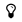
\includegraphics{../manuscript/images/tips.png}\textbf{TIPS} 

Dalam
bahasa C++, tidak terdapat \emph{error handling} terhadap batasan nilai
indeks, apakah indeks tersebut berada di dalam indeks array yang sudah
didefinisikan atau belum. Hal ini merupakan tanggung jawab programmer.
Sehingga jika programmer mengakses indeks yang salah, maka nilai yang
dihasilkan akan berbeda atau rusak karena mengakses alamat memori yang
tidak sesuai.
\end{quotation}
 

\subsubsection*{Contoh  Penanganan Batas Indeks Elemen Array}

Buatlah program beikut ini:

\begin{lstlisting}[language=c++, caption=Penanganan Batas Indeks Elemen Array, label=contoh3-3]
#include <QtCore/QCoreApplication>
#include <iostream>
using namespace std;
int main(int argc, char *argv[])
{
  QCoreApplication a(argc, argv);
  int angka[5];
  angka[0] = 0; //batas bawah array
  angka[4] = 4; //batas atas array
  angka[5] = 5; //indeks melebihi batas
  //program akan HANG
  cout<<angka[5];
  return a.exec();
}
\end{lstlisting}

\textbf{Hasil dan Keterangan:}

\begin{itemize}

\item
  Progarm akan HANG-UP. Hal ini terjadi karena compiler tidak
  bertanggungjawab dengan pengaksesan indeks array yang melebihi batas
  yang dipesankan di memory.
\item
  Mengapa kompiler tidak menampilkan error pada saat kompilasi? Hal ini
  karena secara sintaks, program diatas tidaklah memiliki error
  penulisan. Error yang terjadi pada program diatas adalah runtime
  error, yaitu error yang terjadi / yang bisa dideteksi saat program
  sudah berjalan!
\end{itemize}

\subsection{Inisialisasi Array Satu Dimensi}\label{inisialisasi-array-satu-dimensi}

Array satu dimensi dapat diisi secara langsung ditulis pada program.
Pengisian data seperti itu sering disebut dengan inisialisasi data
array. Cara menginisialisasi data pada array adalah dengan menuliskannya
secara langsung pada source code program. Berikut contohnya:

\begin{lstlisting}[language=c++, numbers=none]
// An array of 5 integers, all elements initialized to 0
int IntegerArray[5] = {0};
\end{lstlisting}

Pada contoh diatas, semua elemen array bertipe integer yang berjumlah 5
buah tersebut diisi dengan nilai 0 semuanya. Cara lain menginisialisasi
array satu dimensi adalah sebagai berikut:

\begin{lstlisting}[language=c++, numbers=none]
// An array of 5 integers initialized to zero
int IntegerArray[5] = { 0, 0, 0, 0, 0 };
\end{lstlisting}

Nah, bagaimana jika kita ingin menginisialisasi elemen terakhirnya saja?
Kita tidak bisa melakukannya secara langsung. Yang harus dilakukan
adalah dengan menginisialisasinya satu-persatu seperti contoh berikut:

\begin{lstlisting}[language=c++, numbers=none]
// An array of 5 integers initialized to zero
int IntegerArray[5] = { 0, 0, 0, 0, 6 };
\end{lstlisting}

Pada contoh diatas, elemen terakhir diinilisasi dengan nilai 6. Kita
tidak bisa langsung mengisi dengan cara
\texttt{int\ IntegerArray{[}5{]}\ =\ \{6\}}, karena jika di isi dengan
cara demikian, maka isi elemen indeks ke-0 bernilai 6, sedangkan elemen
lainnya bernilai 0.

\subsubsection*{Contoh  Inisialisasi Array dengan nilai \textbackslash{}0}

Buatlah program berikut:

\begin{lstlisting}[language=c++, caption=Inisialisasi Array dengan nilai \textbackslash{}0, label=contoh3-4]
#include <QtCore/QCoreApplication>
#include <iostream>
using namespace std;
int main(int argc, char *argv[])
{
  QCoreApplication a(argc, argv);
  int bil[7] = {0}; //inisialisasi 0
  for(int i=0;i<7;i++){
    cout<<"Elemen ke-"<<i<<": "<<bil[i]<<"\n";
  }
  return a.exec();
}
\end{lstlisting}

\textbf{Hasil:}

\begin{lcverbatim}
Elemen ke-0: 0
Elemen ke-1: 1
Elemen ke-2: 2
Elemen ke-3: 3
Elemen ke-4: 4
Elemen ke-5: 5
Elemen ke-6: 6
\end{lcverbatim}

\textbf{Keterangan}

Pada program diatas elemen array bernama bil yang dipesan sebanyak 7
elemen, di inisialisasi dengan nilai 0. Setelah di inisialisasi dengan
nilai 0, maka semua elemen array tersebut juga akan berisi dengan nilai
0. Hal ini dibuktikan dengan cara perulangan semua elemen array dan
ditampilkan dengan \texttt{cout}.

\subsubsection*{Contoh  Inisialisasi Array dua nilai elemen pertama}

Buka Qt Creator dan buat project Qt Console Application baru dengan
nama contoh \ref{contoh3-1}, kemudian tulis kode berikut.

\begin{lstlisting}[language=c++, caption=Inisialisasi Array dua nilai elemen pertama, label=contoh3-5]
#include <QtCore/QCoreApplication>
#include <iostream>
using namespace std;
int main(int argc, char *argv[])
{
  QCoreApplication a(argc, argv);
  int bil[7] = {2,5}; //inisialisasi dua elemen pertama
  for(int i=0;i<7;i++){
    cout<<"Elemen ke-"<<i<<": "<<bil[i]<<"\n";
  }
  return a.exec();
}
\end{lstlisting}

\textbf{Hasil:}

\begin{lcverbatim}
Elemen ke-0: 2
Elemen ke-1: 5
Elemen ke-2: 0
Elemen ke-3: 0
Elemen ke-4: 0
Elemen ke-5: 0
Elemen ke-6: 0
\end{lcverbatim}

\textbf{Keterangan}

Inisialisasi elemen array dapat dilakukan hanya pada dua elemen pertama
saja, hal ini dilakukan dengan cara memberikan dua nilai pertama,
selanjutnya semua elemen lainnya yang tidak di inisialisasi secara
otomatis bernilai 0.

\begin{quotation}
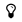
\includegraphics{../manuscript/images/tips.png}\textbf{TIPS}

Untuk
semua array pada C++, inisialisasi satu buah elemen saja pada array akan
membuat semua elemen array lainnya berisi nilai 0.
\end{quotation}
 

\textbf{Contoh:}

\begin{lstlisting}[language=c++, numbers=none]
int angka[100] = {1};
\end{lstlisting}

Maka hasilnya adalah:

\begin{lstlisting}[language=c++, numbers=none]
angka[0] = 1,
angka[1] s/d angka[99] = 0
\end{lstlisting}

Pada array satu dimensi, kita tidak dapat melakukan inisialisasi pada
array melebihi batas jumlah elemen array yang dipesan.

Pada array satu dimensi, kita juga dapat membuat array 1 dimensi tanpa
menyebutkan jumlah elemen array yang dipesan. Namun perlu di ingat bahwa
semua elemen harus di inisialisai terlebih dahulu.

Contoh:

\begin{lstlisting}[language=c++, numbers=none]
int data[5] = {1,2,3,4,5,6}; //error
int data2[] = {10,20}; //terpesan 2 tempat dimemory
\end{lstlisting}

\subsubsection*{Contoh  Tanpa inisialisasi, array langsung ditampilkan}

Tulislah program berikut ini:

\begin{lstlisting}[language=c++, caption=Tanpa inisialisasi array langsung ditampilkan, label=contoh3-6]
#include <QtCore/QCoreApplication>
#include <iostream>
using namespace std;
int main(int argc, char *argv[])
{
  QCoreApplication a(argc, argv);
  char h[5];
  for(int i=0;i<5;i++){
    cout<<"Elemen ke "<<i<<" = "<<h[i]<<endl;
  }
  return a.exec();
  }
\end{lstlisting}

\textbf{Hasil:}

\begin{lcverbatim}
Elemen ke-0: 2
Elemen ke-1: 5
Elemen ke-2: 0
Elemen ke-3: 0
Elemen ke-4: v
\end{lcverbatim}

\textbf{Keterangan}

Pada program C++, elemen array yang sudah dipesan dimemory pasti sudah
berisi data. Namun nilai datanya bersifat acak. Sehingga jika kita
mendeklarasikan sebuah elemen array tanpa di inisialisasi, maka nilai
masing-masing elemen akan bersifat acak juga seperti pada hasil program
diatas. Untuk itulah inisialisasi elemen array sangatlah penting.

\begin{quotation}
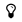
\includegraphics{../manuscript/images/tips.png} \textbf{TIPS}
 
 Inisialisasi pada elemen array yang dideklarsikan \textbf{SANGATLAH
 PENTING} untuk menghindari nilai \textbf{ACAK}!
\end{quotation}


\subsubsection*{Contoh  Penggunaan tipe data enum pada Array satu dimensi}

Buatlah program berikut:

\begin{lstlisting}[language=c++, caption=Penggunaan tipe data enum pada Array satu dimensi, label=contoh3-7]
#include <QtCore/QCoreApplication>
#include <iostream>
using namespace std;
int main(int argc, char *argv[])
{
QCoreApplication a(argc, argv);
enum Hari { Minggu, Senin, Selasa, Rabu, Kamis, Jumat, Sabtu };
int ArrayHari[7] = { 10, 20, 30, 40, 50, 60, 70 };
cout << "Nilai Hari Selasa adalah: " << ArrayHari[Selasa];
return a.exec();
}
\end{lstlisting}

\textbf{Hasil:}

\begin{lcverbatim}
Nilai hari selasa adalah = 30
\end{lcverbatim}

\textbf{Keterangan:}

Pada program diatas, kita membuat sebuah tipe data enum bernama Hari
yang memiliki 7 elemen. Masing-masing elemen \texttt{enum} sama saja
seperti indeks array yaitu \texttt{0-6}. Kemudian kita membuat sebuah
array bernama \texttt{ArrayHari} yang berisi 7 elemen juga dan berisi
nilai \texttt{10-70}. Karena kita memanggil \\
\texttt{ArrayHari{[}Selasa{]}} berarti sama artinya dengan
\texttt{ArrayHari{[}2{]}}. Mengapa 2? Karena indeks Selasa adalah 2.
Sehingga muncullah output berupa 30, karena 30 berada pada indeks ke-2
dari \texttt{ArrayHari}.

Arti dari program diatas menunjukkan kita dapat mengakses indeks
\emph{array} dengan menggunakan \texttt{tipe\ data\ enum}, karena tipe
data \texttt{enum} pada kenyataannya akan dikonversikan kedalam nilai
\texttt{integer}, mulai dari \texttt{0}.

\subsection{Pengalamatan dan Pengkopian Array 1 Dimensi}\label{pengalamatan-dan-pengkopian-array-1-dimensi}

Array tidak bisa disalin begitu saja antara array satu yang ada nilainya
ke array lain yang kosong. Hal ini dikerenakan array bukanlah tipe data
primitif biasa. Array merupakan tipe data referensi dimana data yang
berada didalam elemen array berjumlah lebih dari satu buah dan diakses
dengan menggunakan alamat memory. Compiler C++ akan mencatat alamat
pertama dari indeks pertama array yang kita deklarasikan.

Contoh:

\begin{lstlisting}[language=c++, numbers=none]
int data[5] = {1,2,3,4,5};
\end{lstlisting}

Maka variabel array data tersebut akan dicatat alamat elemen
\texttt{data{[}0{]}} pada memory. Jika kita mengakses elemen keduanya,
yaitu \texttt{data{[}1{]}}, maka compiler akan melakukan kalkulasi untuk
mendapatkan alamat \texttt{data{[}1{]}}, yaitu dengan cara menambahkan
alamat \texttt{data{[}0{]}} dengan lebar tipe data array yang kita
deklarasikan. Pada contoh diatas, kita membuat array bertipe integer.
Karena integer berukuran 4 byte, maka jika \texttt{data{[}0{]}}
beralamat di alamat \texttt{1000}, maka \texttt{data{[}1{]}} beralamat
di \texttt{1000\ +\ 4\ =\ 1004} dan seterusnya.

Lalu bagaimana cara mengkopikan isi elemen array dari satu variabel ke
variable array 1 dimensi lainnya? Kita harus menggunakan cara manual,
yaitu mengkopikan masing-masing elemennya satu persatu dengan perulangan
manual sesuai dengan jumlah elemen array yang dibuat.

\subsubsection*{Contoh  Percobaan Penyalinan Array 1 dimensi}

Buatlah program berikut:

\begin{lstlisting}[language=c++, caption=Percobaan Penyalinan Array 1 dimensi, label=contoh3-8]
#include <QtCore/QCoreApplication>
#include <iostream>
using namespace std;
int main(int argc, char *argv[])
{
  QCoreApplication a(argc, argv);
  int A[6]={1,2,3,4,5,6};
  int B[6];
  B = A;
  return a.exec();
}
\end{lstlisting}

\textbf{Hasil:}

\begin{figure}[htbp]
\centering
\includegraphics[width=0.8\textwidth]{../manuscript/images/capture3-8.PNG}

\end{figure}

\textbf{Keterangan:}

Program tidak bisa dijalankan karena terdapat \textbf{error}, bahwa
array tidak bisa dilakukan operasi assigment. Artinya kita tidak bisa
mengkopi antar array begitu saja.

\subsubsection*{Contoh  Penyalinan Array 1 dimensi dengan Perulangan}

Buatlah program berikut ini:

\begin{lstlisting}[language=c++, caption=Penyalinan Array 1 dimensi dengan Perulangan, label=contoh3-9]
#include <QtCore/QCoreApplication>
#include <iostream>
using namespace std;
int main(int argc, char *argv[])
{
  QCoreApplication a(argc, argv);
  int A[6]={1,2,3,4,5,6};
  int B[6];
  for(int i=0;i<6;i++){
    B[i]=A[i];
  }
  for(int j=0;j<6;j++){
    cout<<B[j]<<endl;
  }
  return a.exec();
}
\end{lstlisting}

\textbf{Hasil:}

\begin{lcverbatim}
1
2
3
4
5
6
\end{lcverbatim}

\textbf{Keterangan:}

\begin{itemize}

\item
  Cara penyalinan array adalah dengan melakukan perulangan sebanyak
  elemen array yang akan disalin dan menyalinnya secara manual
  satu-persatu pada indeks yang sama.
\item
  Kemudian ditampilkan sesuai dengan indeksnya. Elemen array yang
  dikopikan masih tetap memiliki array yang asli. Untuk menghapusnya,
  maka harus dilakukan secara manual.
\end{itemize}

\subsection{Array Multi Dimensi}\label{array-multi-dimensi}

Array multi dimensi berarti array yang kita deklasaikan dapat
dikembangkan ke array dimensi 2 dan seteruanya. Array multi dimensi
merupakan topik yang menarik dalam matematika. Setiap dimensi dalam
array direpresentasikan sebagai sub bagian dalam array. Oleh karena itu,
array dua dimensi array memiliki dua sub bagian, sebuah array
tiga-dimensi memiliki tiga sub bagian dan sebagainya. Sebuah contoh
bentuk nyata yang baik dari array dua dimensi adalah sebuah papan catur.
Satu dimensinya merupakan delapan baris, sedangkan dimensi lainnya
merupakan delapan kolom.

Contoh deklarasi array dua dimensi yang menggambarkan papan catur
adalah:

\begin{lstlisting}[language=c++, numbers=none]
int papan[8][8];
\end{lstlisting}

yang digambarkan dalam bentuk gambar \ref{gambar3-2}:

\begin{figure}[htbp]
\centering
\includegraphics[width=0.8\textwidth]{../manuscript/images/capture3-11.PNG}
\label{gambar3-2}
\caption{Contoh deklarasi array dua dimensi yang menggambarkan papan catur}
\end{figure}

Array dua dimensi sering kali digambarkan/dianalogikan sebagai sebuah
matriks atau bentuk grid. Jika array berdimensi satu hanya terdiri dari
1 baris dan banyak kolom, array berdimensi dua terdiri dari banyak baris
dan banyak kolom yang bertipe sama. Ilustrasi array dua dimensi dapat
dilihat sebagai berikut.

Berikut adalah gambar array berdimensi (baris x kolom = 3 x 4)

\begin{figure}[htbp]
\centering
\includegraphics[width=0.6\textwidth]{../manuscript/images/capture3-12.PNG}
\label{gambar3-3}
\caption{array dimensi 3 x 4}
\end{figure}

\subsection{Deklarasi Array Dua Dimensi}\label{deklarasi-array-dua-dimensi}

\begin{lstlisting}[language=c++, numbers=none]
tipe_data nama_var_array[batas_baris][batas_kolom];
\end{lstlisting}

\textbf{Contoh:}

\begin{lstlisting}[language=c++, numbers=none]
int matriks[3][4];
int matriks2[3][4] = { {5,20,1,11}, {4,7,67,-9}, {9,0,45,3} };
\end{lstlisting}

Array dua dimensi dapat mewakili bentuk suatu matriks, contoh matriks:


$x=
\begin{bmatrix}
8 &5& 9 & 6 & \\
8 & 2 & 1 & 0
\end{bmatrix}$

selanjutnya dapat dideklarasikan sebagai berikut:

\begin{lstlisting}[language=c++]
int x[2][4];
\end{lstlisting}

atau diklarasikan dengan langsung menginisialisasi nilai
elemen-elemen-nya sebagai berikut:

\begin{lstlisting}[language=c++, numbers=none]
int x[2][4]= {{8, 5, 9, 8},{8, 2, 1, 0}}
\end{lstlisting}

Selanjutnya larik dua dimensi x dapat digambarkan sebagai berikut:

\begin{lstlisting}[language=c++, numbers=none]
x[0][0]=8 x[0][1]=5 x[0][2]=9 x[0][3]=8
x[1][0]=8 x[1][1]=2 x[1][2]=1 x[1][3]=0
\end{lstlisting}

Array dua dimensi dapat digunakan untuk menampung tipe data numerik atau
non numerik.

Berikut adalah berbagai bentuk pembuatan array dua dimensi dengan tipe
data numerik ataupun non numerik.

Array dua dimensi bertipe data numerik

\begin{lstlisting}[language=c++, numbers=none]
int matriks[3][5] = {{5,12,17,10,7},
{15,6,25,2,19},
{4,9,20,22,11}};
\end{lstlisting}

Jika data array integer yang diinputkan kurang dari deklarasi

\begin{lstlisting}[language=c++, numbers=none]
int matriks[3][5] = {{5,12,17,10,7},
{15,6,25,2,19},
{4,9 }}; //kurang 3 angka
\end{lstlisting}

Maka tiga data yang kurang akan diisi dengan angka 0

Array 2 dimensi dapat juga digunakan untuk menyimpan data karakter
(character). Pendeklarasian array 2 dimensi character adalah sebagai
berikut:

\begin{lstlisting}[language=c++, numbers=none]
char matriks[3][5] = {{'A','B','C','D','E'},
{'F','G','H','I','J'},
{'K','L','M','N','O'}};
char matriks[3][5] = {"ABCDE",
"FGHIJ",
"KLMNO"};
\end{lstlisting}

Akan ditampilkan sebagai:

\begin{tabular}{|c|c|c|c|c|}
\hline
A &B &C& D& E \\ \hline
F &G &H &I& J \\ \hline
K &L &M& N& O \\ \hline

\end{tabular}

Array 2 dimensi juga dapat dideklarasikan sebagai berikut:

\begin{lstlisting}[language=c++, numbers=none]
char matriks[5][12] = {"Jakarta",
"Bandung",
"Surabaya",
"Semarang",
"Yogyakarta"};
\end{lstlisting}

Array diatas akan ditampilkan sebagai:

\begin{tabular}{|c|c|c|c|c|c|c|c|c|c|c|}
\hline
J & a & k & a & r & t & a & \textbackslash{0} & & & \\ \hline
B & a & n & d & u & n & g & \textbackslash{0} & & & \\ \hline
S & u & r & a & b & a & y & a &\textbackslash{0}  & &\\ \hline
S & e & m & a & r & a & n & g & \textbackslash{0} & & \\ \hline
Y & o & g & y & a & k & a & r & t & a &   \textbackslash{0} \\ \hline

\end{tabular}


Jika jumlah nilai character lebih banyak daripada deklarasi

\begin{lstlisting}[language=c++, numbers=none]
char matriks2[2][2] = {'a','b','c','d','e'};
\end{lstlisting}

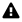
\includegraphics{../manuscript/images/warning.PNG} Akan terjadi ERROR!

\begin{figure}[htbp]
\centering
\includegraphics[width=0.8\textwidth]{../manuscript/images/capture3-10.PNG}

\end{figure}

Jika data array character yang diinputkan kurang dari deklarasi

\begin{lstlisting}[language=c++, numbers=none]
char matriks[3][5] = {{'a','b','c','d','e'},
{'f','g','h','i','j'},
{'k','l' }}; //kurang 3 karakter
\end{lstlisting}

Maka tiga data yang kurang akan diisi dengan karakter NULL atau `\textbackslash{}0'

Jika data array integer yang diinputkan lebih dari deklarasi

\begin{lstlisting}[language=c++, numbers=none]
int matriks[3][5] = {{5,12,17,10,7},
{15,6,25,2,19},
{4,9,20,22,11,14,19 }}; //lebih 2 angka
\end{lstlisting}

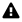
\includegraphics{../manuscript/images/warning.PNG} Matriks yang jumlah datanya lebih akan menyebabkan ERROR


\begin{figure}
\centering
\includegraphics[width=0.8\textwidth]{../manuscript/images/capture3-9.PNG}
\end{figure}




Array 2 dimensi juga dapat dideklarasikan secara dinamis. Dinamis bisa
dilakukan pada baris array 2 dimensi. Namun kita tidak bisa
mendeklarasikan array 2 dimensi secara dinamis pada kolom. Contoh
pendeklarasian baris dinamis adalah :

\begin{lstlisting}[language=c++, numbers=none]
int matriks[][5] = {{5,12,17,10,7},
{15,6,25,2,19},
{4,9,20,22,11}};
\end{lstlisting}

Akan ditampilkan sebagai:

\begin{tabular}{|c|c|c|c|c|}
\hline
5&12&17&10&7 \\ \hline
15&6&25&2&19 \\ \hline
4&9&20&22&11 \\ \hline
\end{tabular}


Contoh matriks dengan deklarasi baris dinamis lainnya:

\begin{lstlisting}[language=c++, numbers=none]
int matriks[][5] = {5,12,17,10,7,
15,6,25,2,19,
4,9,20,22,11,77,88,99};
\end{lstlisting}

Pada contoh diatas, jika kita hitung jumlah datanya adalah 18 buah,
padahal jika kita bagi per lima kolom, maka data 18 akan lebih 3 buah
(18/5 = 3). Sehingga secara otomatis terdapat 3 baris dan sisa 3 buah
data berikutnya akan membuat baris baru. Array dua dimensi tersebut akan
ditampilkan sebagai:


\begin{tabular}{|c|c|c|c|c|}
\hline
5 & 12 & 17 & 10 & 7 \\ \hline
15 & 6 & 25 & 2 & 19 \\ \hline
4 & 9 & 20 & 22 & 11 \\ \hline
77 & 88 & 99 & 0 & 0 \\ \hline

\end{tabular}

\subsubsection{Pengaksesan Array 2 Dimensi}\label{pengaksesan-array-2-dimensi}

Pengaksesan elemen-elemen array 2 dimensi dilakukan dengan cara
perulangan. Perulangan yang dilakukan harus disesuaikan dengan jumlah
dimensinya. Maka array 2 dimensi berarti perulangan yang dilakukan harus
dua kali. Terdapat outer loop yang digunakan untuk mengakses baris array
2 dimensi, dan inner loop yang digunakan untuk mengakses kolom array 2
dimensi.

\subsubsection*{Contoh  Deklarasi dan Menampilkan Array 2 Dimensi}

Buatlah program berikut:

\begin{lstlisting}[language=c++, caption=Deklarasi dan Menampilkan Array 2 Dimensi, label=contoh3-10]
#include <QtCore/QCoreApplication>
#include <iostream>
using namespace std;
int main(int argc, char *argv[])
{
  QCoreApplication a(argc, argv);
  int matriks[3][5] = {{5,12,17,10,7},
  {15,6,25,2,19},
  {4,9,1,5,2}};
  for(int i=0;i<3;i++){
    for(int j=0;j<5;j++){
      cout<<matriks[i][j]<<"\t";
    }
      cout<<endl;
    }
  return a.exec();
}
\end{lstlisting}

\textbf{Hasil:}

\begin{lcverbatim}
51217107
15625219
4 91 52
\end{lcverbatim}


\textbf{Keterangan:}

Program diatas mendeklarasikan sebuah variabel array 2 dimensi bernama
matriks berukuran 3 baris dan 5 kolom. Kemudian matriks tersebut
langsung diinisialisasi dengan data integer sejumlah 15 data. Setelah
diinisialisasi kemudian dilakukan pengaksesan terhadap array 2 dimensi
tersebut dengan cara melakukan dua buah perulangan. Perulangan pertama
disebut outer loop yang digunakan untuk mengakses indeks baris variabel
matriks, sedangkan perulangan kedua disebut inner loop yang digunakan
untuk mengakses indeks kolom variabel matriks. Kemudian untuk
menampilkan data nya digunakan perintah cout dan untuk setiap data
elemen array diberikan karakter tab yang digunakan untuk memberi jarak
antar output data. Karakter tab pada bahasa C menggunakan escape
character `\textbackslash{}t'.

\subsubsection*{Contoh  Penyalinan Array 2 Dimensi ke Array 2 Dimensi lainnya}

Misalkan terdapat array 2 dimensi sebagai berikut
matriks\texttt{{[}3{]}{[}5{]}}

\begin{tabular}{|c|c|c|c|c|}
\hline
1 & 2 & 3 & 4 & 5 \\ \hline
6 & 7 & 8 & 9 & 10 \\ \hline
11 & 12 & 13 & 14 & 15 \\ \hline

\end{tabular}

Buatlah program berikut:

\begin{lstlisting}[language=c++, caption=Penyalinan Array 2 Dimensi ke Array 2 Dimensi lainnya, label=contoh3-11]
#include <QtCore/QCoreApplication>
#include <iostream>
using namespace std;
int main(int argc, char *argv[])
{
  QCoreApplication a(argc, argv);
  int matriks[3][5]={{1,2,3,4,5},{6,7,8,9,10},{11,12,13,14,15}};
  int matrikshasil[3][5];
  for(int i=0;i<3;i++){
    for(int j=0;j<5;j++){
      matrikshasil[i][j] = matriks[i][j];
    }
  }
  for(int i=0;i<3;i++){
    for(int j=0;j<5;j++){
      cout<<matrikshasil[i][j]<<"\t";
    }
    cout<<endl;
  }
  return a.exec();
}
\end{lstlisting}

\textbf{Hasil:}

\begin{lcverbatim}
12345
678910
1112131416
\end{lcverbatim}

\textbf{Keterangan:}

Program diatas menyalin data dari matriks 2 dimensi ke matriks 2 dimensi
lainnya dengan menggunakan perulangan bertingkat. Perulangan bertingkat
memiliki 2 buah loop, yang pertama (\emph{outer loop}) digunakan untuk
mengakses baris matriks, dan inner loop digunakan untuk mengakses kolom
matriks. Kemudian untuk masing-masing elemen matriks dimasukkan kedalam
variabel array matrikshasil tepat pada baris dan kolom yang sesuai.

\subsubsection*{Contoh  Penyalinan array 2 dimensi ke dalam array 1 dimensi.}

Buatlah program berikut ini:

\begin{lstlisting}[language=c++, caption=Penyalinan array 2 dimensi ke dalam array 1 dimensi, label=contoh3-12]
#include <QtCore/QCoreApplication>
#include <iostream>
using namespace std;
int main(int argc, char *argv[])
{
  QCoreApplication a(argc, argv);
  int matriks[3][5]={{1,2,3,4,5},{6,7,8,9,10},{11,12,13,14,15}};
  int matrikshasil[15];
  int counter=-1;
  for(int i=0;i<3;i++){
    for(int j=0;j<5;j++){
      counter++;
      matrikshasil[counter] = matriks[i][j];
    }
  }
  for(int i=0;i<15;i++){
    cout<<matrikshasil[i]<<endl;
  }
  return a.exec();
}
\end{lstlisting}

\textbf{Hasil:}

\begin{lcverbatim}
1
2
3
4
5
6
7
8
9
10
11
12
13
14
15
\end{lcverbatim}

\textbf{Keterangan:}

\begin{itemize}

\item
  Untuk menyalin array 2 dimensi ke 1 dimensi, maka harus diperlukan
  sebuah array 1 dimensi baru yang berukuran total sesuai dengan hasil
  perkalian antara ukuran baris matriks dua dimensi dikalikan kolomnya.
  Misal array 2 dimensi berukuran 3 x 5, maka harus dibuat array 1
  dimensi berukuran minimal 15.
\item
  Kemudian untuk mengkopikan dari array 2 dimensi matriks ke array 1
  dimensi matrikshasil, harus dilakukan perulangan sesuai dengan baris
  dan kolom matriks. Indeks array matrikshasil diperoleh dari penambahan
  nilai counter yang diinisialisasi dari -1, dan berjalan mulai dari 0
  sampai dengan 14.
\end{itemize}

\subsection{Akses Array 2 dimensi}
 
Cara Pengaksesan Array dapat dilakukan dengan 2 cara:

\begin{enumerate}
\item Pengaksesan Baris demi Baris

Cara ini menelusuri elemen array dua dimensi per dimulai dari baris
pertama lalu kekanan sesuai dengan jumlah kolomnya. Setelah eleman dalam
baris tersebut habis, maka penelusuran akan berganti baris ke baris
berikutnya dan demikian seterusnya. Cara ini membutuhkan 2 buah loop,
dimana outer loop digunakan untuk mengakses indeks baris, dan inner loop
digunakan untuk mengakses indeks kolom.

Berikut adalah contohnya:

\begin{lstlisting}[language=c++, caption=Pengaksesan Baris demi Baris, label=contoh3-13]
#include <QtCore/QCoreApplication>
#include <iostream>
using namespace std;
int main(int argc, char *argv[])
{
QCoreApplication a(argc, argv);
int A[2][3]={{1,2,3},{4,5,6}};
for(int baris=0;baris<2;baris++){
for(int kolom=0;kolom<3;kolom++){
cout<<A[baris][kolom]<<"\t";
}
cout<<endl;
}
return a.exec();
}
\end{lstlisting}

\textbf{Hasil:}

\begin{lcverbatim}
1 2 3
4 5 6
\end{lcverbatim}

\item Pengaksesan Kolom demi Kolom

Cara ini menelusuri elemen array dua dimensi per dimulai dari kolom
pertama lalu kebawah sesuai dengan jumlah barisnya. Setelah eleman dalam
kolom tersebut habis, maka penelusuran akan berganti kolom ke kolom
berikutnya dan demikian seterusnya. Cara ini membutuhkan 2 buah loop,
dimana outer loop digunakan untuk mengakses indeks kolom, dan inner loop
digunakan untuk mengakses indeks baris.

\textbf{Contoh:}

\begin{lstlisting}[language=c++, caption=Pengaksesan Kolom demi Kolom, label=contoh3-14]
#include <QtCore/QCoreApplication>
#include <iostream>
using namespace std;
int main(int argc, char *argv[])
{
QCoreApplication a(argc, argv);
int A[2][3]={{1,2,3},{4,5,6}};
for(int kolom=0;kolom<3;kolom++){
for(int baris=0;baris<2;baris++){
cout<<A[baris][kolom]<<"\t";
}
cout<<endl;
}
return a.exec();
}
\end{lstlisting}

\textbf{Hasil:}

\begin{lcverbatim}
1 4
2 5
3 6
\end{lcverbatim}

\end{enumerate}







\section{String}\label{string}

\index{String}String adalah kumpulan dari nilai-nilai karakter yang berurutan dalam
bentuk satu dimensi, nilai string ini haruslah ditulis didalam tanda
petik dua (") misalnya: ``ini string''. Suatu nilai string disimpan di
memori dengan diakhiri oleh nilai ``\textbackslash{}''0(null), misalnya nilai string
``ANTO'' disimpan dimemori dalam bentuk

\begin{tabular}{|c|c|c|c|c|}
\hline
A & N & T & 0 & \textbackslash{0}\\ \hline
\end{tabular}


Dengan mengetahui nilai string diakhiri oleh nilai `\textbackslash{}0', maka akhir
nilai dari suatu string dapat dideteksi.

Untuk mendeklarasikan sebuah string terdapat dua cara:

\begin{enumerate}


\item
  Menggunakan \index{array of character}array of character yang sering disebut 
  \index{C-style}C-style string
\item
  Menggunakan tipe data string pada C++
\end{enumerate}

\subsection{Array of Character}\label{array-of-character}

Cara menggunakan array of character sama seperti mendeklarasikan
variabel bertipe array namun bertipe data character seperti yang sudah
dijelaskan pada bagian-bagian sebelumnya. Array of character memiliki
sifat-sifat array lainnya yaitu bersifat statis dan letaknya berurutan
di dalam memory komputer. String berjenis array of character selalu
dibuat dengan menggunakan array satu dimensi yang dapat terdiri dari
karakter-karakter yang ditulis dengan menggunakan tanda petik tunggal
(') atau satu kesatuan string yang ditulis dengan tanda petik ganda
('').

\subsubsection*{Contoh pendeklarasian array of character}

\begin{lstlisting}[language=c++, numbers=none]
char nama[6]; //tanpa inisialisasi
char nama2[6] = "anton"; //langsung diinisialisasi
char nama2[6] = {'a','n','t','o','n'}; //langsung diinisialisasi
\end{lstlisting}

Pada sebuah string, terdapat karakter \texttt{\textbackslash{}0} yang
dapat digunakan untuk mengetahui kapan berakhirnya suatu string. Berikut
adalah contoh penggunaaanya.

\subsubsection*{Contoh  Penggunaan karakter \textbackslash{0}}

Buatlah program berikut:

\begin{lstlisting}[language=c++, caption=Penggunaan karakter \textbackslash{0}, label=contoh3-15]
#include <QtCore/QCoreApplication>
#include <iostream>
using namespace std;
int main(int argc, char *argv[])
{
  QCoreApplication a(argc, argv);
  char string[100]="String";
  int K;
  for(K=0;string[K]!='\0';K++)
    cout<<string[K];
  return a.exec();
}
\end{lstlisting}

\textbf{Hasil:}

\begin{lcverbatim}
String
\end{lcverbatim}

\textbf{Keterangan:}

Program diatas dapat mengetahui kapan berakhirnya suatu string, dalam
arti kita dapat mengetahui panjang suatu string dengan melakukan
perulangan untuk setiap karakter yang ada pada array sampai ditemukannya
katakter `\textbackslash{}0'.

\subsubsection*{Contoh  String tanpa karakter \textbackslash{0}}

Buatlah program berikut:

\begin{lstlisting}[language=c++, caption=String tanpa karakter \textbackslash{0}, label=contoh3-16]
#include <QtCore/QCoreApplication>
#include <iostream>
using namespace std;
int main(int argc, char *argv[])
{
  QCoreApplication a(argc, argv);
  char string[6]="String";
  int K;
  for(K=0;string[K]!='\0';K++)
    cout<<string[K];
  return a.exec();
}
\end{lstlisting}

\textbf{Hasil:}

\begin{figure}[htbp]
\centering
\includegraphics[width=0.8\textwidth]{../manuscript/images/capture2-7.PNG}

\end{figure}

\textbf{Keterangan:}

Terlihat bahwa kita tidak bisa membuat array fa character tepat sesuai
dengan jumlah karakter yang kita inisialisasikan. Jika dilihat kata
``String'' berjumlah 6 huruf, sedangkan kita sudah mendeklarasikan
variabel \texttt{string{[}6{]}} namun ternyata jumlah elemennya masih
dianggap terlalu sedikit. Hal ini terjadi karena minimal kita harus
mengalokasikan sejumlah 7 buah elemen. Elemen ke-7 digunakan untuk
menyimpan tanda akhir string atau karakter \textbackslash0 tersebut.

\subsubsection*{Contoh  Mengisi Array of Character}

Buatlah program berikut:

\begin{lstlisting}[language=c++, caption=Mengisi Array of Character, label=contoh3-17]
#include <QtCore/QCoreApplication>
#include <iostream>
using namespace std;
int main(int argc, char *argv[])
{
  QCoreApplication a(argc, argv);
  char buffer[50] = {'\0'};
  cout << "Isi data string: ";
  cin >> buffer;
  cout << "Hasil data string: " << buffer << endl;
  return a.exec();
}
\end{lstlisting}

\textbf{Hasil:}
\begin{lcverbatim}
Isi data string: Wachid
hasil data string: Wachid
\end{lcverbatim}


\textbf{Keterangan:}

\begin{itemize}

\item
  Pada program diatas kita mendeklarasikan variabel array of string
  bernama buffer yang berukuran 6 elemen. Variabel buffer diatas
  merupakan variabel berjenis string C-style yang diinisialisasi dengan
  karakter \textbackslash{0} atau karakter\index{NULL} NULL.
\item
  Problem lainnya adalah jika kita menginputkan data string yang
  mengandung spasi, maka cin hanya akan membaca data string sebelum
  spasi saja.
\end{itemize}

\textbf{Contoh:}

\begin{lstlisting}[language=c++, numbers=none]
Isi data string: Nur Wachid
hasil data string: Wachid
\end{lstlisting}

\subsubsection*{Contoh  Pengisian variabel array of character dengan maksimum jumlah karakter.}

Tulislah program berikut:

\begin{lstlisting}[language=c++, caption=Pengisian variabel array of character dengan maksimum jumlah
karakter, label=contoh3-18]
#include <QtCore/QCoreApplication>
#include <iostream>
using namespace std;
int main(int argc, char *argv[])
{
  QCoreApplication a(argc, argv);
  char buffer[50] = {'\0'};
  cout << "Isi data string: ";
  cin.get(buffer,49); //ambil sebanyak 50 karakter atau diakhiri tanda enter
  cout << "Hasil data string: " << buffer << endl;
  return a.exec();
}
\end{lstlisting}

\textbf{Hasil:}
\begin{lcverbatim}
Isi data string: Nur Wachid
hasil data string: Nur Wachid
\end{lcverbatim}


\textbf{Keterangan:}

Pada contoh program diatas, kita menggunakan perintah
\texttt{cin.get(buffer,49)}. Perintah diatas ``memaksa'' agar perintah
\texttt{cin} mengambil semua data inputan ke dalam variabel buffer
sampai sejumlah 49 karakter. Jika karakter yang diinputkan lebih dari 50
karakter, maka otomatis karakter yang disimpan kedalam variabel buffer
hanyalah berjumlah 50 karakter pertama saja.

\section{Fungsi-fungsi String}\label{fungsi-fungsi-string}

Bahasa C++ menggunakan fungsi-fungsi pustaka yang disediakan untuk
mengoperasikan suatu nilai string yang dimasukkan dalam file header
string.h. Beberapa fungsi string yang terdapat pada header string.h
adalah sebagai berikut:

\begin{lstlisting}[language=c++, numbers=none]
strlen()
\end{lstlisting}

Berfungsi untuk menentukkan panjang suatu nilai string.

Bentuk umum:
\texttt{int\ strlen(\textless{}identifier\ string\textgreater{});}

\begin{lstlisting}[language=c++, numbers=none]
length()
\end{lstlisting}

Berfungsi untuk menentukan panjang suatu nilai tipe data class string

Bentuk umum method:
\texttt{\textless{}nama\_var\_string\textgreater{}.length();}

\subsubsection*{Contoh  Penggunaan fungsi strlen()}

Buatlah program berikut ini:

\begin{lstlisting}[language=c++, caption=Penggunaan fungsi strlen(), label=contoh3-19]
#include <QtCore/QCoreApplication>
#include <iostream>
using namespace std;
int main(int argc, char *argv[])
{
  QCoreApplication a(argc, argv);
  char data[100];
  cout<<"Masukkan kalimat apapun yang anda sukai (max 100 huruf): ";
  cin.get(data,99);
  cout<<"panjang huruf adalah: "<<strlen(data)<<" karakter";
  return a.exec();
}
\end{lstlisting}

\textbf{Hasil:}

\begin{lcverbatim}
Masukkan kalimat apapun
yang anda sukai (max 100 huruf): Nur Wachid 
panjang huruf adalah: 10 karakter
\end{lcverbatim}
 

\textbf{Keterangan:}

Fungsi strlen menerima satu parameter yang hanya bertipe array of
character. Fungsi ini tidak bisa menerima parameter berupa tipe data C++
string.

\subsubsection*{Contoh  Penggunaan fungsi length pada tipe data string C++}

Buatlah program berikut ini:

\begin{lstlisting}[language=c++, caption=Penggunaan fungsi length pada tipe data string C++, label=contoh3-20]
#include <QtCore/QCoreApplication>
#include <iostream>
#include <string>
using namespace std;
int main(int argc, char *argv[])
{
  QCoreApplication a(argc, argv);
  string data2;
  cout<<"Masukkan kalimat apapun yang anda sukai (max 100 huruf): ";
  getline(cin,data2);
  cout<<"panjang huruf adalah: "<<data2.length()<<" karakter";
  return a.exec();
}
\end{lstlisting}

\textbf{Hasil:}

\begin{lcverbatim}
Masukkan kalimat apapun yang anda sukai
(max 100 huruf): Nur Wachid 
panjang huruf adalah: 10 karakter
\end{lcverbatim}
 

\textbf{Keterangan}

\begin{itemize}

\item
  Program diatas tidak menggunakan array of character, melainkan
  menggunakan tipe data C++ \texttt{class\ string}. Tipe data ini
  spesial karena berupa tipe data object oriented. Untuk menggunakan
  tipe data ini kita harus menginclude-kan
  \texttt{\#include\ \textless{}string\textgreater{}} pada bagian
  \emph{preprocessor directive}.
\item
  Kemudian untuk mengakses panjang karakternya digunakan method (fungsi)
  dari object string bernama \texttt{length()}. Fungsi \texttt{length}
  sama dengan fungsi \texttt{strlen} yaitu mengambil jumlah karakter
  dalam string tersebut.
\end{itemize}

\subsection{strcpy() dan strncpy()}\label{strcpy-dan-strncpy}

Dalam bahasa C++, untuk menyalin nilai suatu string tidak dapat langsung
menuliskannya seperti halnya kompiler lain, sehingga proses menyalin
atau mengerjakan suatu nilai string ke variabel string yang lain
diperlukan suatu fungsi pustaka yang bernama \texttt{strcpy()}.

\begin{enumerate}

\item
  Bentuk umum:
  \texttt{void\ strcpy(\textless{}stringhasil\textgreater{},\textless{}stringsumber\textgreater{});}
\item
  Bentuk umum:
  \texttt{void\ strncpy(\textless{}stringhasil\textgreater{},\textless{}stringsumber\textgreater{});}
\end{enumerate}

\subsubsection*{Contoh  Penggunaan fungsi strcpy()}

Buatlah program berikut ini:

\begin{lstlisting}[language=c++, caption=Penggunaan fungsi strcpy(), label=contoh3-21]
#include <QtCore/QCoreApplication>
#include <iostream>
#include <string>
using namespace std;
int main(int argc, char *argv[])
{
  QCoreApplication a(argc, argv);
  char data[100] = {'\0'};
  char data2[]="STRING";
  strcpy(data,data2);
  cout<<"string pertama: "<<data<<"\n";
  cout<<"string kedua : "<<data2;
  return a.exec();
}
\end{lstlisting}

\textbf{Hasil:}
\begin{lcverbatim}
String pertama : STRING
String Kedua : STRING
\end{lcverbatim}


\textbf{Keterangan:}

\begin{itemize}
\item
  Program diatas digunakan untuk mengkopikan nilai dari array of
  character data ke data2 dengan menggunakan perintah \texttt{strcpy}.
  Hal itu terbukti dengan hasil akhir dimana string pertama dan kedua
  bernilai sama, yaitu ``STRING''.
\item
  Jika variabel sesumber lebih besar daripada variabel hasil,
  \texttt{trcpy\ ()} akan error karena melebihi buffer. Untuk melindungi
  hal ini, digunakan fungsi \texttt{strncpy\ ()} Fungsi ini dapat
  memberikan parameter jumlah maksimum karakter untuk penyalinan.
  \texttt{strncpy\ ()} akan menyalin sampai karakter null pertama atau
  jumlah maksimum. Contoh Error:

  \begin{itemize}
  
  \item
    \texttt{char\ data{[}5{]}\ =\ \{\textquotesingle{}\textbackslash{}0\textquotesingle{}\};}
  \item
    \texttt{char\ data2{[}{]}="STRING";}
  \end{itemize}
\item
  Hal ini terjadi karena data2 berjumlah 6 karakter, sedangkan data
  berjumlah 5 karakter. Jadi ketika data2 dikopikan ke data, maka akan
  terjadi error karena tempatnya kurang.
\end{itemize}

\subsubsection*{Contoh  Penggunaan fungsi strncpy()}

Buatlah program beriku:

\begin{lstlisting}[language=c++, caption=Penggunaan fungsi strncpy(), label=contoh3-22]
#include <QtCore/QCoreApplication>
#include <iostream>
#include <string>
using namespace std;
int main(int argc, char *argv[])
{
  QCoreApplication a(argc, argv);
  char data[6] = {'\0'};
  char data2[]="STRINGKU";
  strncpy(data,data2,5);
  cout<<"string pertama: "<<data<<"\n";
  cout<<"string kedua : "<<data2;
  return a.exec();
}
\end{lstlisting}

\textbf{Hasil:}
\begin{lcverbatim}
 String pertama : STRING
 String Kedua : STRINGKU
\end{lcverbatim}


\textbf{Keterangan:}

\begin{itemize}

\item
  Fungsi \texttt{strncpy} dapat digunakan untuk menyalin dari satu array
  of character ke array of character lainnya dengan memberikan penanda
  batas maksimal penyalinan. Pada contoh diatas, string ``STRINGKU''
  hendak disalin ke variabel data yang hanya berisi 6 elemen. Karena
  fungsi \texttt{strncpy} hanya dibatasi menyalin 5 karakter saja, maka
  yang tersalin adalah \texttt{STRIN} saja.
\item
  Karakter ke-6 pada variabel data digunakan untuk menyimpan karakter
 NULL atau \textbackslash0.
\end{itemize}

\subsection{strcat()}\label{strcat}

\textbf{Bentuk umum}:
\texttt{strcat(\textless{}string\ hasil\textgreater{},\ \textless{}string\ sumber\textgreater{});}

String dalam C++ tidak bisa digabungkan begitu saja dengan menggunakan
operator + seperti pada bahasa pemrograman Pascal. Jika dipaksakan
menggunakan operator + akan ditampilkan pesan kesalahan sebagai berikut
ini.

\subsubsection*{Contoh  Penggunaan fungsi strcat()}

Buatlah program beriku:

\begin{lstlisting}[language=c++, caption=Penggunaan fungsi strcat(), label=contoh3-23]
#include <QtCore/QCoreApplication>
#include <iostream>
#include <string>
using namespace std;
int main(int argc, char *argv[])
{
  QCoreApplication a(argc, argv);
  char str[6] = "anton";
  char str2[7];
  char str3[14];
  str3 = str + str2;
  return a.exec();
}
\end{lstlisting}

\textbf{Hasil:}

\begin{figure}[htbp]
\centering
\includegraphics[width=0.8\textwidth]{../manuscript/images/capture3-6.PNG}

\end{figure}

\textbf{Keterangan:}

Opearator + tidak bisa digunakan untuk menggabungkan dua buah string.
Untuk menggabungkan dua string, digunakan fungsi \texttt{strcat()}.

\subsubsection*{Contoh  Penggunaan fungsi strcat()}

Buatlah program berikut:

\begin{lstlisting}[language=c++, caption=Penggunaan fungsi strcat(), label=contoh3-24]
#include <QtCore/QCoreApplication>
#include <iostream>
#include <string>
using namespace std;
int main(int argc, char *argv[])
{
  QCoreApplication a(argc, argv);
  char string1[100]="Kami kelompok ";
  char string2[]=" belajar Qt C++";
  strcat(string1,string2);
  cout<<"Jadi gabungannya adalah: "<<string1;
  return a.exec();
}
\end{lstlisting}

\textbf{Hasil:}

\begin{lcverbatim}
Jadi gabungannya adalah:
Kami kelompok belajar Qt C++
\end{lcverbatim}


\textbf{Keterangan:}

\begin{itemize}

\item
  Program diatas menggunakan fungsi \texttt{strcat} dimana fungsi
  tersebut akan menggabungkan dua buah string. Parameter string pertama
  juga digunakan untuk menampung string gabungan kedua string tersebut.
  Sehingga pada akhirnya variabel string1 lah yang ditampilkan ke layar.
\item
  Variabel \texttt{string1} diberi ukuran 100 karena jika tidak diberi
  ukuran elemen maka \texttt{string1} tidak bisa memperbesar ukurannya
  di memory komputer sehingga akan menyebabkan program \textbf{HANG}.
\end{itemize}

\begin{quotation}
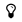
\includegraphics{../manuscript/images/tips.png}\textbf{TIPS}

Beberapa fungsi yang \texttt{\#include\ string.h} dan dapat digunakan
untuk memanipulasi \emph{array of character} adalah:

\emph{strrev()}

Bentuk umum: \texttt{strrev(string)}

Digunakan untuk membalik susunan string, misal: anton menjadi notna

\emph{strlwr()}

Bentuk umum: \texttt{strlwr(string)}

Digunakan untuk mengubah string menjadi huruf kecil semua

\emph{strupr}

Bentuk umum: \texttt{strupr(string)}

Digunakan untuk mengubah string menjadi huruf besar semua

\emph{strchr()}

Bentuk umum: \texttt{strchr(stringsumber,karakter\ yang\ dicari)}

Dalam bahasa C++ disediakan suatu fungsi pustaka yaitu \texttt{strchr()}
untuk mencari nilai suatu karakter yang ada di suatu string. Hasil dari
fungsi ini adalah alamat letak dari karakter pertama di nilai string
yang sama dengan karakter yang dicari.

\emph{strcmp()}

Bentuk umum: \texttt{strcmp(string1,string2);}

Untuk membandingkan dua nilai string tidak bisa menggunakan operator
hubungan, karena operator tersebut tidak untuk operasi string. Untuk
membandingkan dua nilai string kita gunakan fungsi pustaka
\texttt{strcmp()} dengan hasil sebagai berikut:

\begin{itemize}

\item
Hasil \textless{} 0, Jika string1 \textless{} string2
\item
Hasil = 0, Jika string1 = string2
\item
Hasil \textgreater{} 0, Jika string1 \textgreater{} string2
\end{itemize}
\end{quotation}


\subsection{Fungsi mengubah string menjadi numerik dan sebaliknya}\label{fungsi-mengubah-string-menjadi-numerik-dan-sebaliknya}

Pada bahasa C++ tipe data \emph{array of character} bisa dikonversi
menjadi \texttt{numerik} dan sebaliknya numerik bisa dikonversi menjadi
\texttt{array\ of\ character}. Caranya adalah
\texttt{\#include\ \textless{}stdlib\textgreater{}}. Fungsi-fungsi
konversi dari string ke numerik adalah:

\begin{lstlisting}[language=c++, numbers=none]
atoi() //untuk mengubah string menjadi int
atof() //untuk mengubah string menjadi float
atol() //untuk mengubah string menjadi long int
\end{lstlisting}

Sedangkan kebalikannya, fungsi untuk mengubah numerik menjadi string
adalah:

\begin{lstlisting}[language=c++, numbers=none]
itoa() //untuk mengubah int menjadi string
ltoa() //untuk mengubah long int menjadi string
ultoa() //untuk mengubah unsigned long menjadi string
\end{lstlisting}

Fungsi diatas menerima parameter
\texttt{\textless{}var\ numerik\textgreater{}},
\texttt{\textless{}var\ array\ of\ character\textgreater{}}, dan
\texttt{\textless{}basis\ bilangan\textgreater{}}

\subsection{Class string pada C++}\label{class-string-pada-c}

C++ library standar memiliki kelas string yang membuat bekerja dengan
string lebih mudah dengan menyediakan satu set encapsulasi dari data,
dan fungsi untuk memanipulasi data \index{String}string. Kelas ini dikenal dengan
\texttt{std::} string yang dapat menangani rincian alokasi memori dan
membuat kopi string, atau menempatkan mereka di memory dengan lebih
mudah.

\subsubsection*{Contoh  Pembuatan variabel string C++, penyalinan string, dan
penggabungan string}

Buatlah program berikut:

\begin{lstlisting}[language=c++, caption=Pembuatan variabel string C++ penyalinan string dan
penggabungan string, label=contoh3-25]
#include <QtCore/QCoreApplication>
#include <iostream>
#include <string>
using namespace std;
int main(int argc, char *argv[])
{
  QCoreApplication a(argc, argv);
  string str1("Ini string C++");
  cout<<"Isi str1 = "<<str1<<endl;
  //salin isi str1 ke str2
  string str2;
  str2 = str1;
  cout<<"Isi str2 = "<<str2<<endl;
  //ubah str2
  str2 = "Hallo, ";
  //buat strhasil dan isi dgn gabungan dari str1 dan str2
  string strhasil;
  strhasil = str2 + str1;
  cout<<strhasil;
  return a.exec();
}
\end{lstlisting}

\textbf{Hasil:}

\begin{lcverbatim}
Isi str1 : Ini string C++
Isi str1 : Ini string C++
Isi str1 : Ini string C++
Halo, Ini string C++
\end{lcverbatim}

\textbf{Keterangan:}

\begin{itemize}

\item
  Tanpa perlu dipelajari lebih dalam, kita dapat melihat bahwa class
  string pada C++ jelas jauh lebih cepat penggunaannya dan mudah dalam
  pembuatan serta penyalinan seperti semudah mengoperasikan variabel
  bertipe integer saja. Demikian pula, \emph{concatenating}
  (penggabungan) dua string dapat dilakukan dengan hanya menambahkan
  mereka, sama juga seperti kita akan melakukan penjumlahan dengan
  integer apapun.
\item
  Syarat untuk dapat menggunakan class string adalah harus
  mengincludekan \texttt{\#include\ \textless{}string\textgreater{}},
  seperti yang dapat dilihat pada kode program diatas.
\end{itemize}
\begin{quotation}
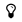
\includegraphics{../manuscript/images/tips.png} \textbf{TIPS} 
 
 Class
 string memiliki beberapa fitur / manfaat, yaitu: 
\begin{itemize}
\item Mengurangi kesulitan dalam upaya penciptaan dan
memanipulasi string
\item Meningkatkan stabilitas aplikasi
yang sedang diprogram dalam pengelolaan dan alokasi memori internal
\item Mudah dalam menyalin, memotong, menemukan, dan
penghapusan string
\item Memberikan kesempatan pada
programmer untuk lebih fokus pada pengembangan aplikasi daripada
kesulitan dalam manipulasi string
\end{itemize} 
 
\end{quotation}


\subsubsection*{Contoh  Penggunaan class string untuk manipulasi data}

Buatlah program berikut:

\begin{lstlisting}[language=c++, caption=Penggunaan class string untuk manipulasi data, label=contoh3-26]
#include <QtCore/QCoreApplication>
#include <iostream>
#include <string>
using namespace std;
int main(int argc, char *argv[])
{
  QCoreApplication a(argc, argv);
  //buat var nama dgn C-style string
  char nama[10] = "Halooooooo";
  //buat var string dan diisi nilai dari var nama
  string nama_copy(nama);
  cout<<nama_copy<<endl;
  //buat var nama2 dan kopikan isinya ke nama2_copy melalui konstruktor
  string nama2 = "saya belajar";
  string nama2_copy(nama2);
  cout<<nama2_copy<<endl;
  //buat var nama35 yg diisi nilai dari nama tapi hanya 5 huruf saja
  string nama35(nama,5);
  cout<<nama35<<endl;
  //buat var ulang yg diisi huruf 'C' sebanyak 10 buah
  string ulang(10,'a');
  cout<<ulang;
  return a.exec();
}
\end{lstlisting}

\textbf{Hasil:}

 \begin{lcverbatim}
 Halooooooo
 saya belajar
 C
 \end{lcverbatim}

\textbf{Keterangan:}

Dapat dilihat langsung pada baris komentar program diatas.

\subsubsection*{Contoh  Penggabungan string dengan menggunakan class string}

Buatlah program berikut:

\begin{lstlisting}[language=c++, caption=Penggabungan string dengan menggunakan class string, label=contoh3-27]
#include <QtCore/QCoreApplication>
#include <iostream>
#include <string>
using namespace std;
int main(int argc, char *argv[])
{
  QCoreApplication a(argc, argv);
  string satu("Percobaan 1 ");
  string dua("Percobaan 2 ");
  satu += dua;
  cout<<satu<<endl;
  string tampung = "Percobaan tampung";
  satu.append("Percobaan 3 ");
  satu.append(tampung);
  cout<<satu;
  return a.exec();
}
\end{lstlisting}

\textbf{Hasil:}
\begin{lcverbatim}
Percobaan 1 Percobaan 2
Percobaan 1 Percobaan 2 Percobaan 3 Percebaan tampung
\end{lcverbatim}


\textbf{Keterangan:}

\begin{itemize}

\item
  Pada program diatas, terdapat dua buah variabel bertipe string, yaitu
  \texttt{satu} dan \texttt{dua}. Tipe data string tidak mendukung
  penggabungan string dengan mudah yaitu dengan menggunakan operator +.
  Pada contoh diatas, variabel satu ditambah isinya dengan variabel dua
  dan disimpan kembali pada variabel satu. Sehingga variabel satu berisi
  string gabungan ``Percobaan 1 Percobaan 2''.
\item
  Kemudian dibuat suatu variabel tampung yang kemudian juga digabungkan
  kedalam variabel satu. Cara penggabungan (concatenation) string dapat
  dilakukan juga dengan cara kedua, yaitu dengan menggunakan
  \texttt{method\ append}. \texttt{Method\ append} ini dimiliki oleh
  semua variabel bertipe class string dan dapat langsung digunakan
  dengan memasukkan parameter bertipe string juga.
\end{itemize}

\subsubsection*{Contoh  Pengaksesan isi nilai class string}

Buatlah program berikut:

\begin{lstlisting}[language=c++, caption=Pengaksesan isi nilai class string, label=contoh3-28]
#include <QtCore/QCoreApplication>
#include <iostream>
#include <string>
using namespace std;
int main(int argc, char *argv[])
{
  QCoreApplication a(argc, argv);
  string satu("Indonesia Raya");
  for(size_t i=0;i<satu.length();i++){
    cout<<satu[i]<<endl;
  }
  cout<<endl;
  cout<<"C-sytle: "<<satu.c_str();
  return a.exec();
}
\end{lstlisting}

\textbf{Hasil:}

\begin{lcverbatim}
I
n
d
o
n
e
s
i
a


R
a
y
a

C-style: Indonesia Raya
\end{lcverbatim}

\textbf{Keterangan:}

\begin{itemize}

\item
  Variabel string yang bertipe class string juga memiliki sifat yang
  sama dengan variabel string dengan model C-string style. Keduanya
  merupakan gabungan dari karakter-karakter yang berbentuk array
  berdimensi satu. Sehingga jika kita memiliki variabel string satu
  seperti pada program, kita dapat mengakses semua elemen-elemen
  karakter penyusun string tersebut dengan menggunakan perulangan dan
  kemudian kita akses indeks dari masing-masing elemen array
  characternya.
\item
  Pada bagian kedua, kita juga bisa mengkonversi dari tipe data class
  string menjadi tipe data array of character atau tipe data C-style
  string dengan menggunakan method dari class string, yaitu
  \texttt{c\_str()}.
\end{itemize}

\subsubsection*{Contoh  Menemukan substring pada sebuah string besar}

Tulislah program berikut ini:

\begin{lstlisting}[language=c++, caption=Menemukan substring pada sebuah string besar, label=contoh3-29]
#include <QtCore/QCoreApplication>
#include <iostream>
#include <string>
using namespace std;
int main(int argc, char *argv[])
{
  QCoreApplication a(argc, argv);
  string strSample ("Kata pak Hari, \"hari ini matahari cerah sekali!\"");
  cout << "Contoh string adalah: " << endl;
  cout << strSample << endl << endl;
  // Temukan kata "hari"
  size_t nOffset = strSample.find ("hari", 0);
  // Cek apakah ketemu?
  if (nOffset != string::npos)
    cout << "Ketemu pertama kata \"hari\" pada offset " << nOffset;
  else
    cout << "Substring tidak ditemukan" << endl;
    cout << endl << endl;
    cout << "Mencari semua kata substring \"hari\"" << endl;
    size_t nSubstringOffset = strSample.find ("hari", 0);
  while (nSubstringOffset != string::npos)
  {
    cout << "Kata \"hari\" ada di offset " << nSubstringOffset << endl;
    // Pencarian dilanjutkan ke karakter berikutnya dst
    size_t nSearchOffset = nSubstringOffset + 1;
    nSubstringOffset = strSample.find ("hari", nSearchOffset);
  }
  cout << endl;
  cout << "Mencari semua karakter 'a'" << endl;
  const char chCharToSearch = 'a';
  size_t nCharacterOffset = strSample.find (chCharToSearch, 0);
  while (nCharacterOffset != string::npos)
  {
    cout << "'" << chCharToSearch << "' ditemukan";
    cout << " pada posisi " << nCharacterOffset << endl;
    //pencarian dilanjutkan
    size_t nCharSearchOffset = nCharacterOffset + 1;
    nCharacterOffset = strSample.find(chCharToSearch,nCharSearchOffset);
  }
  return a.exec();
}
\end{lstlisting}

\textbf{Hasil:}

\begin{lcverbatim}
Contoh string adalah:
Kata pak Hari, "hari ini matahari cerah sekali!"
Ketemu pertama kata "hari" pada offset 16
Mencari semua kata substring "hari"
Kata "hari" ada di offset 16
Kata "hari" ada di offset 29
Mencari semua karakter 'a'
'a' ditemukan pada posisi 1
'a' ditemukan pada posisi 3
'a' ditemukan pada posisi 6
'a' ditemukan pada posisi 10
'a' ditemukan pada posisi 17
'a' ditemukan pada posisi 26
'a' ditemukan pada posisi 28
'a' ditemukan pada posisi 30
'a' ditemukan pada posisi 37
'a' ditemukan pada posisi 43
\end{lcverbatim}

\textbf{Keterangan:}

\begin{itemize}

\item
  Program diatas membuat sebuah variabel string bernama strSample yang
  diisi dengan kalimat : ``Kata pak Hari, ``hari ini matahari cerah
  sekali!''\,''. Kemudian program akan mencari kata ``hari'' yang
  pertama ditemukan pada kalimat tersebut dengan menggunakan method
  find(\texttt{\textless{}kata\ yang\ dicari\textgreater{}},\texttt{\textless{}posisi\ indeks\ dimulainya\ pencarian\textgreater{}}).
  Method ini bersifat case-sensitive sehingga kata ``Hari'' dengan
  ``hari'' berbeda. Pencarian dimulai dari huruf pertama, sehingga kata
  ``hari'' ditemukan pada huruf ke 16, bukan ke-9, karena karakter ke-9
  kata ``Hari'' menggunakan huruf besar.
\item
  Pencarian berikutnya adalah pencarian semua kata ``hari''. Karena kata
  ``hari'' ada lebih dari satu buah, maka pencarian harus diloop, karena
  method find membutuhkan indeks mulainya pencarian. Untuk setiap kata
  ``hari'' yang ditemukan, kemudian ditampilkan posisi indeksnya ke
  layar.
\item
  Selain dapat menerima parameter berupa substring, method find juga
  dapat menerima parameter berupa character dengan proses pencarian yang
  sama dengan proses pencarian dengan parameter substring.
\end{itemize}

\subsubsection*{Contoh  Membalik kata / kalimat.}

Tulislah program berikut ini:

\begin{lstlisting}[language=c++, caption=Membalik kata / kalimat, label=contoh3-30]
#include <QtCore/QCoreApplication>
#include <iostream>
#include <string>
#include <algorithm>
using namespace std;
int main(int argc, char *argv[])
{
QCoreApplication a(argc, argv);
string strSample ("String ini akan dibalik!");
cout << "String asli: " << endl;
cout << strSample << endl << endl;
reverse (strSample.begin (), strSample.end ());
cout << "Setelah dibalik: " << endl;
cout << strSample;
return a.exec();
}
\end{lstlisting}

\textbf{Hasil:}

\begin{lcverbatim}
String asli:
String ini akan dibalik!
Setelah dibalik:
!kilabid naka ini gnirtS
\end{lcverbatim}

\textbf{Keterangan:}

Untuk membalik kalimat bertipe string, kita harus menggunakan \index{library}library
header \index{algoritm}algoritm, sehingga kita harus mengincludekan library tersebut
\texttt{\#include\ \textless{}algorithm\textgreater{}}. Setelah itu
untuk menggunakannya kita gunakan perintah
\emph{reverse}(\texttt{\textless{}indeks\ string\ pertam\textgreater{}},\texttt{\textless{}indeks\ string\ terakhir\textgreater{}}).
Perintah reverse tersebut akan benar-benar mengganti string asli menjadi
terbalik, sehingga variable string kita akan berubah berisi kalimat yang
sudah terbalik.

\subsubsection*{Contoh  Konversi huruf besar dan kecil.}

Tulislah program berikut ini:

\begin{lstlisting}[language=c++, caption=Konversi huruf besar dan kecil, label=contoh3-31]
#include <QtCore/QCoreApplication>
#include <iostream>
#include <string>
#include <algorithm>
using namespace std;
int main(int argc, char *argv[])
{
  QCoreApplication a(argc, argv);
  cout << "Masukkan sebuah string: " << endl;
  string strInput;
  getline (cin, strInput);
  transform(strInput.begin(),strInput.end(),strInput.begin(),(int(*)(int))toupper);
  cout << "Hasil konversi ke huruf besar: " << endl;
  cout << strInput << endl << endl;
  transform
  (strInput.begin(),strInput.end(),strInput.begin(),(int(*)(int))tolower);
  cout << "Hasil konversi ke huruf kecil: " << endl;
  cout << strInput << endl << endl;
  return a.exec();
}
\end{lstlisting}

\textbf{Hasil:}

\begin{lcverbatim}
Masukkan sebuah string:
Ini KoK tulisaNya AlaY BaNGet yA!
Hasil konversi ke huruf besar:
INI KOK TULISANYA ALAY BANGET YA!

Hasil konversi ke huruf kecil:
ini kok tulisanya alay banget ya!
\end{lcverbatim}

\textbf{Keterangan:}

Program diatas menunjukkan function transform pada library algoritm
dapat digunakan untuk mengkonversi string dari besar ke kecil dan dari
kecil ke besar.
